\documentclass[11pt,a4paper]{report}
\usepackage[textwidth=37em,vmargin=30mm]{geometry}
\usepackage{calc,xunicode,amsmath,amssymb,paralist,enumitem,tabu,booktabs,datetime2,xeCJK,xeCJKfntef,listings}
\usepackage{tocloft,fancyhdr,tcolorbox,xcolor,graphicx,eso-pic,xltxtra,xelatexemoji}

\newcommand{\envyear}[0]{2025}
\newcommand{\envdatestr}[0]{2025-10-11}
\newcommand{\envfinaldir}[0]{webdb/2025/20251011/final}

\usepackage[hidelinks]{hyperref}
\hypersetup{
    colorlinks=false,
    pdfpagemode=FullScreen,
    pdftitle={Web Digest - \envdatestr}
}

\setlength{\cftbeforechapskip}{10pt}
\renewcommand{\cftchapfont}{\rmfamily\bfseries\large\raggedright}
\setlength{\cftbeforesecskip}{2pt}
\renewcommand{\cftsecfont}{\sffamily\small\raggedright}

\setdefaultleftmargin{2em}{2em}{1em}{1em}{1em}{1em}

\usepackage{xeCJK,xeCJKfntef}
\xeCJKsetup{PunctStyle=plain,RubberPunctSkip=false,CJKglue=\strut\hskip 0pt plus 0.1em minus 0.05em,CJKecglue=\strut\hskip 0.22em plus 0.2em}
\XeTeXlinebreaklocale "zh"
\XeTeXlinebreakskip = 0pt


\setmainfont{Brygada 1918}
\setromanfont{Brygada 1918}
\setsansfont{IBM Plex Sans}
\setmonofont{JetBrains Mono NL}
\setCJKmainfont{Noto Serif CJK SC}
\setCJKromanfont{Noto Serif CJK SC}
\setCJKsansfont{Noto Sans CJK SC}
\setCJKmonofont{Noto Sans CJK SC}

\setlength{\parindent}{0pt}
\setlength{\parskip}{8pt}
\linespread{1.15}

\lstset{
	basicstyle=\ttfamily\footnotesize,
	numbersep=5pt,
	backgroundcolor=\color{black!5},
	showspaces=false,
	showstringspaces=false,
	showtabs=false,
	tabsize=2,
	captionpos=b,
	breaklines=true,
	breakatwhitespace=true,
	breakautoindent=true,
	linewidth=\textwidth
}






\newcommand{\coverpic}[2]{
    % argv: itemurl, authorname
    Cover photo by #2~~(\href{#1}{#1})
}
\newcommand{\makeheader}[0]{
    \begin{titlepage}
        % \newgeometry{hmargin=15mm,tmargin=21mm,bmargin=12mm}
        \begin{center}
            
            \rmfamily\scshape
            \fontspec{BaskervilleF}
            \fontspec{Old Standard}
            \fontsize{59pt}{70pt}\selectfont
            WEB\hfill DIGEST
            
            \vfill
            % \vskip 30pt
            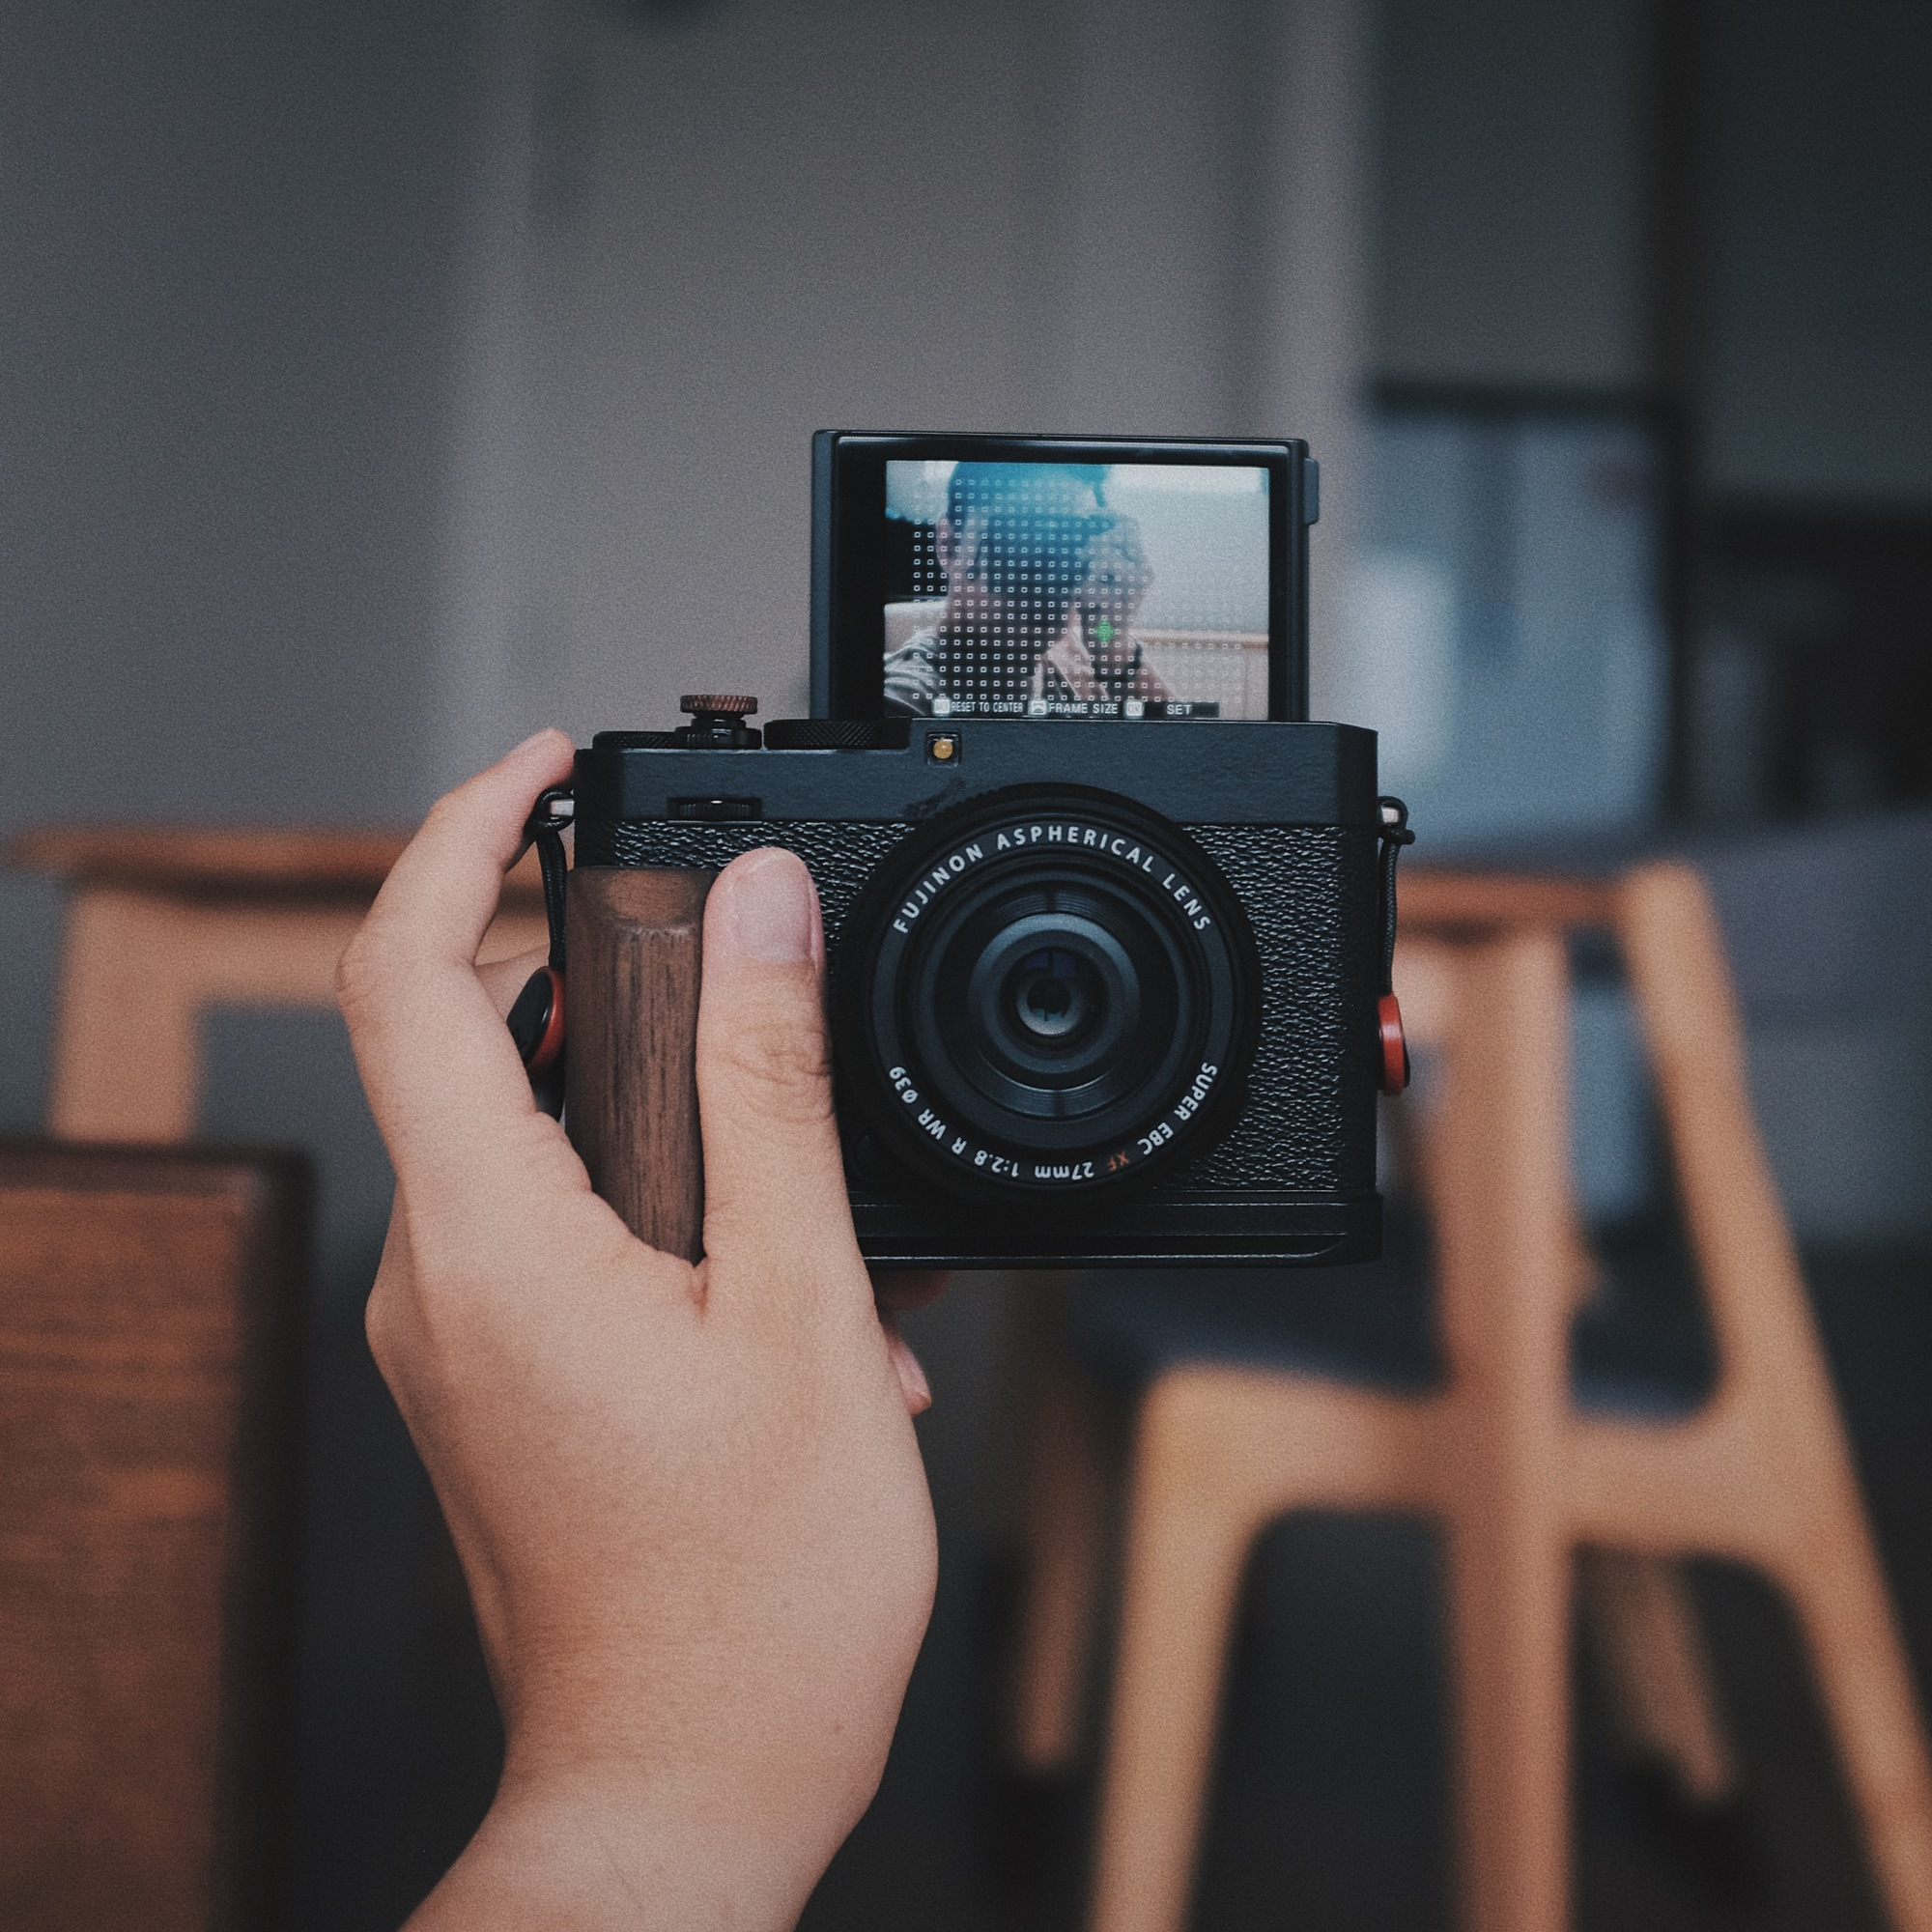
\includegraphics[width=\linewidth]{\envfinaldir/coverpic-prod.jpg}\par
            % \vskip 30pt
            \vfill

            \normalsize\rmfamily\scshape
            \copyright{} The Web Digest Project \hfill\large \envdatestr
        \end{center}
    \end{titlepage}
    % \restoregeometry
}
\newcommand{\simplehref}[1]{%
    \textcolor{blue!80!green}{\href{#1}{#1}}%
}
\renewcommand{\contentsname}{\center\Huge\sffamily\bfseries Contents\par\vskip 20pt}
\newcounter{ipartcounter}
\setcounter{ipartcounter}{0}
\newcommand{\ipart}[1]{
    % \vskip 20pt
    \clearpage
    \stepcounter{ipartcounter}
    \phantomsection
    \addcontentsline{toc}{chapter}{#1}
    % \begin{center}
    %     \Huge
    %     \sffamily\bfseries
    %     #1
    % \end{center}
    % \vskip 20pt plus 7pt
}
\newcounter{ichaptercounter}
\setcounter{ichaptercounter}{0}
\newcommand{\ichapter}[1]{
    % \vskip 20pt
    \clearpage
    \stepcounter{ichaptercounter}
    \phantomsection
    \addcontentsline{toc}{section}{\numberline{\arabic{ichaptercounter}}#1}
    \begin{center}
        \Huge
        \sffamily\bfseries
        #1
    \end{center}
    \vskip 20pt plus 7pt
}
\newcommand{\entrytitlefont}[1]{\subsection*{\raggedright\Large\sffamily\bfseries#1}}
\newcommand{\entryitemGeneric}[2]{
    % argv: title, url
    \parbox{\linewidth}{
        \entrytitlefont{#1}\par\vskip 5pt
        \footnotesize\ttfamily\mdseries
        \simplehref{#2}
    }\vskip 11pt plus 11pt minus 1pt
}
\newcommand{\entryitemGithub}[3]{
    % argv: title, url, desc
    \parbox{\linewidth}{
        \entrytitlefont{#1}\par\vskip 5pt
        \footnotesize\ttfamily\mdseries
        \simplehref{#2}\par\vskip 5pt
        \small\rmfamily\mdseries#3
    }\vskip 11pt plus 11pt minus 1pt
}
\newcommand{\entryitemAp}[3]{
    % argv: title, url, desc
    \parbox{\linewidth}{
        \entrytitlefont{#1}\par\vskip 5pt
        \footnotesize\ttfamily\mdseries
        \simplehref{#2}\par\vskip 5pt
        \small\rmfamily\mdseries#3
    }\vskip 11pt plus 11pt minus 1pt
}
\newcommand{\entryitemHackernews}[3]{
    % argv: title, hnurl, rawurl
    % \parbox{\linewidth}{
    %     \entrytitlefont{#1}\par\vskip 5pt
    %     \footnotesize\ttfamily\mdseries
    %     \simplehref{#3}\par
    %     \textcolor{black!50}{\href{#2}{#2}}
    % }\vskip 11pt plus 11pt minus 1pt
    \begin{minipage}{\linewidth}
            \entrytitlefont{#1}\par\vskip 5pt
            \footnotesize\ttfamily\mdseries
            \simplehref{#3}\par
            \textcolor{black!50}{\href{#2}{#2}}
    \end{minipage}\par\vskip 11pt plus 11pt minus 1pt
}







\begin{document}

\makeheader

\tableofcontents\clearpage




\ipart{Developers}
\ichapter{Hacker News}
\entryitemTwoLinks{Liquid Glass Is Cracked, and Usability Suffers in iOS 26}{https://news.ycombinator.com/item?id=45544044}{https://www.nngroup.com/articles/liquid-glass/}

\entryitemTwoLinks{I built physical album cards with NFC tags to teach my son music discovery}{https://news.ycombinator.com/item?id=45543475}{https://fulghum.io/album-cards}

\entryitemTwoLinks{Google, Meta and Microsoft to stop showing political ads in the EU}{https://news.ycombinator.com/item?id=45542145}{https://www.politico.eu/article/eu-political-ad-rules-google-meta-microsoft-big-tech-kick-in/}

\entryitemTwoLinks{The illegible nature of software development talent}{https://news.ycombinator.com/item?id=45541600}{https://surfingcomplexity.blog/2025/10/08/the-illegible-nature-of-software-development-talent/}

\entryitemTwoLinks{It's OpenAI's world, we're just living in it}{https://news.ycombinator.com/item?id=45541125}{https://stratechery.com/2025/its-openais-world-were-just-living-in-it/}

\entryitemTwoLinks{Regarding the Compact}{https://news.ycombinator.com/item?id=45540989}{https://president.mit.edu/writing-speeches/regarding-compact}

\entryitemTwoLinks{Boring Company cited for almost 800 environmental violations in Las Vegas}{https://news.ycombinator.com/item?id=45540585}{https://www.propublica.org/article/elon-musk-boring-company-violations-fines-vegas-loop}

\entryitemTwoLinks{"Vibe code hell" has replaced "tutorial hell" in coding education}{https://news.ycombinator.com/item?id=45540313}{https://blog.boot.dev/education/vibe-code-hell/}

\entryitemTwoLinks{You can't build tcc from Nixpkgs if you are in the UK}{https://news.ycombinator.com/item?id=45540011}{https://github.com/NixOS/nixpkgs/issues/444342}

\entryitemTwoLinks{Ryanair flight landed at Manchester airport with six minutes of fuel left}{https://news.ycombinator.com/item?id=45539943}{https://www.theguardian.com/business/2025/oct/10/ryanair-flight-landed-at-manchester-airport-with-six-minutes-of-fuel-left-flight-log-suggests}

\entryitemTwoLinks{The Molecular Basis of Long Covid Brain Fog}{https://news.ycombinator.com/item?id=45539845}{https://www.yokohama-cu.ac.jp/english/news/20251001takahashi.html}

\entryitemTwoLinks{Notes on switching to Helix from Vim}{https://news.ycombinator.com/item?id=45539609}{https://jvns.ca/blog/2025/10/10/notes-on-switching-to-helix-from-vim/}

\entryitemTwoLinks{Google Safe Browsing incident}{https://news.ycombinator.com/item?id=45538760}{https://www.statichost.eu/blog/google-safe-browsing/}

\entryitemTwoLinks{Igalia, Servo, and the Sovereign Tech Fund}{https://news.ycombinator.com/item?id=45538137}{https://www.igalia.com/2025/10/09/Igalia,-Servo,-and-the-Sovereign-Tech-Fund.html}

\entryitemTwoLinks{OpenGL: Mesh shaders in the current year}{https://news.ycombinator.com/item?id=45537890}{https://www.supergoodcode.com/mesh-shaders-in-the-current-year/}

\entryitemTwoLinks{Nobel Peace Prize 2025: María Corina Machado}{https://news.ycombinator.com/item?id=45536700}{https://www.nobelprize.org/prizes/peace/2025/summary/}

\entryitemTwoLinks{Show HN: I invented a new generative model and got accepted to ICLR}{https://news.ycombinator.com/item?id=45536694}{https://discrete-distribution-networks.github.io/}

\entryitemTwoLinks{Datastar: Lightweight hypermedia framework for building interactive web apps}{https://news.ycombinator.com/item?id=45536618}{https://data-star.dev/}

\entryitemTwoLinks{I tracked Amazon's Prime Day prices. We've been played}{https://news.ycombinator.com/item?id=45536531}{https://www.washingtonpost.com/technology/2025/10/09/amazon-prime-day-prices/}

\entryitemTwoLinks{A story about bypassing air Canada's in-flight network restrictions}{https://news.ycombinator.com/item?id=45536325}{https://ramsayleung.github.io/en/post/2025/a\_story\_about\_bypassing\_air\_canadas\_in-flight\_network\_restrictions/}\ichapter{Phoronix}
\entryitemGeneric{\hskip 0pt{}Linux Now Disabling TPM Bus Encryption By Default For Performance Reasons}{https://www.phoronix.com/news/Linux-Default-Disable-TPM2-HMAC}

\entryitemGeneric{\hskip 0pt{}AMD ROCm 7.0.2 Released With Radeon RX 9060 Officially Supported}{https://www.phoronix.com/news/AMD-ROCm-7.0.2-Released}

\entryitemGeneric{\hskip 0pt{}Python 3.14 Performance Looking Good In Benchmarks}{https://www.phoronix.com/review/python-314-benchmarks}

\entryitemGeneric{\hskip 0pt{}NVIDIA Posts Latest Linux Driver Patches For Open-Source vGPU Support}{https://www.phoronix.com/news/NVIDIA-vGPU-RFC-v2}

\entryitemGeneric{\hskip 0pt{}Microsoft Hyper-V Support Further Improved With Linux 6.18}{https://www.phoronix.com/news/Linux-6.18-Hyper-V}

\entryitemGeneric{\hskip 0pt{}GCC Patches Posted For C++26 SIMD Support}{https://www.phoronix.com/news/GCC-CPP26-SIMD-Patches}

\entryitemGeneric{\hskip 0pt{}New Input Drivers Merged For Linux 6.18}{https://www.phoronix.com/news/Linux-6.18-Input}

\entryitemGeneric{\hskip 0pt{}Shotcut 25.10 Video Editor Rolling Out More AI-Powered Functionality}{https://www.phoronix.com/news/Shotcut-25.10-Beta}

\entryitemGeneric{\hskip 0pt{}Intel's Lead Engineer For Linux Performance Monitoring Is Leaving The Company}{https://www.phoronix.com/news/Kan-Liang-Leaving-Intel}


\ipart{Developers~~~~(zh-Hans)}
\ichapter{Solidot}
\entryitemGeneric{\hskip 0pt{}研究发现让大模型中毒非常容易}{https://www.solidot.org/story?sid=82515}

\entryitemGeneric{\hskip 0pt{}微软开发者披露臭名昭著的 FCKGW 密钥来历}{https://www.solidot.org/story?sid=82514}

\entryitemGeneric{\hskip 0pt{}英特尔重新思考其开源战略}{https://www.solidot.org/story?sid=82513}

\entryitemGeneric{\hskip 0pt{}日全食期间鸟类行为发生改变}{https://www.solidot.org/story?sid=82512}

\entryitemGeneric{\hskip 0pt{}天文学家使用引力透镜发现最小的暗天体}{https://www.solidot.org/story?sid=82511}

\entryitemGeneric{\hskip 0pt{}裸鼹鼠长寿的秘密可能在于其 DNA 修复机制}{https://www.solidot.org/story?sid=82510}

\entryitemGeneric{\hskip 0pt{}GitHub 正将其基础设施迁移到 Azure}{https://www.solidot.org/story?sid=82509}

\entryitemGeneric{\hskip 0pt{}英国央行对 AI 泡沫破裂发出警告}{https://www.solidot.org/story?sid=82508}

\entryitemGeneric{\hskip 0pt{}空客 A320 交付量超过波音 737}{https://www.solidot.org/story?sid=82507}

\entryitemGeneric{\hskip 0pt{}日本公司本月将把酿酒设备送到国际空间站}{https://www.solidot.org/story?sid=82506}

\entryitemGeneric{\hskip 0pt{}DC 漫画称不会支持 AI 创作}{https://www.solidot.org/story?sid=82505}

\entryitemGeneric{\hskip 0pt{}互联网档案馆被命令在比利时屏蔽部分电子书的访问}{https://www.solidot.org/story?sid=82504}

\entryitemGeneric{\hskip 0pt{}Ubuntu 25.10 'Questing Quokka' 释出}{https://www.solidot.org/story?sid=82503}

\entryitemGeneric{\hskip 0pt{}黄金价格首次突破每盎司 4000 美元}{https://www.solidot.org/story?sid=82502}

\entryitemGeneric{\hskip 0pt{}Fedora 43 将 /boot 分区容量从 1GB 增加到 2GB}{https://www.solidot.org/story?sid=82501}

\entryitemGeneric{\hskip 0pt{}Starlink 每天有 1-2 颗重返大气层}{https://www.solidot.org/story?sid=82500}

\entryitemGeneric{\hskip 0pt{}Salesforce 拒绝为被盗的客户数据支付赎金}{https://www.solidot.org/story?sid=82499}

\entryitemGeneric{\hskip 0pt{}研究认为 BMI 指数不能反映一个人是否健康}{https://www.solidot.org/story?sid=82498}

\entryitemGeneric{\hskip 0pt{}8 月赴美留学生同比下降 19\%}{https://www.solidot.org/story?sid=82497}

\entryitemGeneric{\hskip 0pt{}OpenAI 今年内签署的 AI 计算交易已高达 1 万亿美元}{https://www.solidot.org/story?sid=82496}\ichapter{V2EX}
\entryitemGeneric{\hskip 0pt{}[Solana] 2025.10.11}{https://www.v2ex.com/t/1164331}

\entryitemGeneric{\hskip 0pt{}[Apple] iPhone17 Pro 充电控制问题}{https://www.v2ex.com/t/1164330}

\entryitemGeneric{\hskip 0pt{}[加密货币] f*******k}{https://www.v2ex.com/t/1164329}

\entryitemGeneric{\hskip 0pt{}[Solana] 抄底,管他是不是底!}{https://www.v2ex.com/t/1164328}

\entryitemGeneric{\hskip 0pt{}[Solana] 浇给~}{https://www.v2ex.com/t/1164327}

\entryitemGeneric{\hskip 0pt{}[加密货币] 年度大插针来了,接接接!}{https://www.v2ex.com/t/1164325}

\entryitemGeneric{\hskip 0pt{}[Solana] 本来觉得买 v 币是支持 v 站,但其实钱都被炒作的人赚走了。其实 Livid 没赚什么钱}{https://www.v2ex.com/t/1164324}

\entryitemGeneric{\hskip 0pt{}[分享发现] Claude Code 配合 CCR(Claude Code Router)和 Gemini Balance 实现无限续杯}{https://www.v2ex.com/t/1164323}

\entryitemGeneric{\hskip 0pt{}[Claude] ClaudeCode. + glm4.6 你的评价是什么}{https://www.v2ex.com/t/1164322}

\entryitemGeneric{\hskip 0pt{}[Telegram] End of the free internet 自由互联网的消亡 By Pavel Durov 20251010}{https://www.v2ex.com/t/1164321}

\entryitemGeneric{\hskip 0pt{}[奇思妙想] 有几个公网 ip 和上下行对称的 1G 网络能干点啥}{https://www.v2ex.com/t/1164320}

\entryitemGeneric{\hskip 0pt{}[问与答] 如何关闭烦人的 win11 升级提示}{https://www.v2ex.com/t/1164319}

\entryitemGeneric{\hskip 0pt{}[程序员] 支付宝小游戏真垃圾!服了}{https://www.v2ex.com/t/1164318}

\entryitemGeneric{\hskip 0pt{}[职场话题] 关于搞技术——``搞技术没前途''}{https://www.v2ex.com/t/1164317}

\entryitemGeneric{\hskip 0pt{}[分享发现] 体会到了当老板的快感, AI 给足了我情绪价值}{https://www.v2ex.com/t/1164316}

\entryitemGeneric{\hskip 0pt{}[Python] 𝜋thon ( Python 3.14)}{https://www.v2ex.com/t/1164315}

\entryitemGeneric{\hskip 0pt{}[iPhone] 升级到 iPhone 17 Pro 的体验, iOS 26 拖后腿?}{https://www.v2ex.com/t/1164310}

\entryitemGeneric{\hskip 0pt{}[上海] 在上海 K11 被带 2 个妞精神小伙的特斯拉新款 Y 开门杀了。。对方车主只愿意赔偿一百块}{https://www.v2ex.com/t/1164309}

\entryitemGeneric{\hskip 0pt{}[macOS] macOS 26 系统中在 Chrome 中使用来自 ``信息''、``邮件'' 的验证码,被禁用了}{https://www.v2ex.com/t/1164308}

\entryitemGeneric{\hskip 0pt{}[Solana] 又有两个地址抛了!快抄底!都要 6 开头了!}{https://www.v2ex.com/t/1164307}

\entryitemGeneric{\hskip 0pt{}[问与答] 个人站怎么添加广告,获得收入}{https://www.v2ex.com/t/1164306}

\entryitemGeneric{\hskip 0pt{}[成都] 帮 表妹(摄影师)找个程序员对象}{https://www.v2ex.com/t/1164302}

\entryitemGeneric{\hskip 0pt{}[程序员] 超火的 AI 手办生图 APP 自动构建流程分享给大家}{https://www.v2ex.com/t/1164301}

\entryitemGeneric{\hskip 0pt{}[问与答] 领导让我做一个 AI 自动化测试接口的智能体...}{https://www.v2ex.com/t/1164300}

\entryitemGeneric{\hskip 0pt{}[分享发现] 中国 14 日起将对美国船舶收取船舶特别港务费作为报复}{https://www.v2ex.com/t/1164299}

\entryitemGeneric{\hskip 0pt{}[分享创造] [自荐] OneClip:轻快不打扰的 Mac 剪贴板工具(诚恳求反馈)}{https://www.v2ex.com/t/1164298}

\entryitemGeneric{\hskip 0pt{}[Apple] 备份恢复导致山姆 APP 增加新的绑定设备}{https://www.v2ex.com/t/1164296}

\entryitemGeneric{\hskip 0pt{}[投资] 有没有稳赚不亏的理财方式}{https://www.v2ex.com/t/1164295}

\entryitemGeneric{\hskip 0pt{}[问与答] 使用 chatgpt 网页版,经常卡死,有啥好的解决方案不?}{https://www.v2ex.com/t/1164294}

\entryitemGeneric{\hskip 0pt{}[Apple] 港版 iphone17promax 有 apple care 的情况下不贴膜可以吗}{https://www.v2ex.com/t/1164293}

\entryitemGeneric{\hskip 0pt{}[VPS] 如果你有空闲服务器那么你可以看看这个}{https://www.v2ex.com/t/1164292}

\entryitemGeneric{\hskip 0pt{}[Solana] 卖了九个吃灰的路由器终于凑够了一个钻石,还额外往流动池里注了一点点}{https://www.v2ex.com/t/1164290}

\entryitemGeneric{\hskip 0pt{}[生活] 撸空投!}{https://www.v2ex.com/t/1164289}

\entryitemGeneric{\hskip 0pt{}[Go 编程语言] PerfTest — 轻量级高性能开源压测工具,支持 HTTP/1/2/3 与 WebSocket,还能分布式集群压测}{https://www.v2ex.com/t/1164288}

\entryitemGeneric{\hskip 0pt{}[问与答] 老电脑升级,求个建议}{https://www.v2ex.com/t/1164287}

\entryitemGeneric{\hskip 0pt{}[分享创造] StillRoot:让 AI 对话沉淀为笔记的第二大脑,求大家给点反馈/意见/建议}{https://www.v2ex.com/t/1164286}

\entryitemGeneric{\hskip 0pt{}[职场话题] 申请的苹果电脑被老板截胡,我差点和人事吵起来}{https://www.v2ex.com/t/1164285}

\entryitemGeneric{\hskip 0pt{}[Android] 在国内 Android 上如何同时使用 Gemini 和 Google Maps}{https://www.v2ex.com/t/1164283}

\entryitemGeneric{\hskip 0pt{}[分享创造] 写了一个 FinalShell 加解密工具,欢迎使用}{https://www.v2ex.com/t/1164282}

\entryitemGeneric{\hskip 0pt{}[分享创造] StillRoot:让 AI 对话沉淀为笔记的第二大脑,求 10 人内测反馈}{https://www.v2ex.com/t/1164281}

\entryitemGeneric{\hskip 0pt{}[程序员] 存储涨价了是因为做存储/内存的公司盈利更多了吗}{https://www.v2ex.com/t/1164280}

\entryitemGeneric{\hskip 0pt{}[Apple] 17PM 哪款膜比较好,那种大几百的 ar 膜靠谱嘛}{https://www.v2ex.com/t/1164278}

\entryitemGeneric{\hskip 0pt{}[问与答] 为什么 Chrome 不做侧边栏呢?就行 Arc 一样 侧边栏 tab 感觉很舒服}{https://www.v2ex.com/t/1164276}

\entryitemGeneric{\hskip 0pt{}[分享创造] 用 Svelte 复刻了一个划词翻译 Tampermonkey 脚本}{https://www.v2ex.com/t/1164275}

\entryitemGeneric{\hskip 0pt{}[生活] 怎么会有这样的租房合同?}{https://www.v2ex.com/t/1164274}

\entryitemGeneric{\hskip 0pt{}[酷工作] 远程办公: Python 架构师, 985 学历, 30 岁以内,发 USDT}{https://www.v2ex.com/t/1164273}

\entryitemGeneric{\hskip 0pt{}[宽带症候群] [实测] 深圳电信宽带新产品,不给公网 ip,但是给开端口,是下一代的解决方案吗?}{https://www.v2ex.com/t/1164272}

\entryitemGeneric{\hskip 0pt{}[宽带症候群] [后续 2] 泉州联通案件的近期情况,以及 10 月 13 日(15:00)开庭|地点:泉州鲤城法院}{https://www.v2ex.com/t/1164270}

\entryitemGeneric{\hskip 0pt{}[程序员] vscode copilot 的补全是不是不太行?}{https://www.v2ex.com/t/1164268}

\entryitemGeneric{\hskip 0pt{}[分享创造] 做了一个直播工具,类似 Owncast 但是更轻量}{https://www.v2ex.com/t/1164265}


\ipart{Generic News}







\clearpage
\leavevmode\vfill
\footnotesize

Copyright \copyright{} 2023-2025 Neruthes and other contributors.

This document is published with CC BY-NC-ND 4.0 license.

The entries listed in this newsletter may be copyrighted by their respective creators.

This newsletter is generated by the Web Digest project.

The newsletters are also delivered via Telegram channel \CJKunderline{\href{https://t.me/webdigestchannel}{https://t.me/webdigestchannel}}.\\
RSS feed is available at \CJKunderline{\href{https://webdigest.pages.dev/rss.xml}{https://webdigest.pages.dev/rss.xml}}.

This newsletter is available in PDF at
\CJKunderline{\href{https://webdigest.pages.dev/}{https://webdigest.pages.dev/}}.

The source code being used to generate this newsletter is available at\\
\CJKunderline{\href{https://github.com/neruthes/webdigest}{https://github.com/neruthes/webdigest}}.

This newsletter is also available in
\CJKunderline{\href{http://webdigest.pages.dev/readhtml/\envyear/WebDigest-20251011.html}{HTML}} and
\CJKunderline{\href{https://github.com/neruthes/webdigest/blob/master/markdown/\envyear/WebDigest-20251011.md}{Markdown}}.


\coverpic{https://unsplash.com/photos/monument-valley-at-sunrise-with-sun-flare-XZWInejJTCM}{Tom Donders}


\end{document}
